\documentclass[11pt]{scrartcl}
%%
%
% This is a poster template with latex macros and using
% the University of Florida Logo.  For further information
% on making postscript, resizeing, and printing the poster file
% please see web site 
% http://www.phys.ufl.edu/~pjh/posters/poster_howto.html
% 
% N.B. This format is cribbed from one obtained from the University
% of Karlsruhe, so some macro names and parameters are in German
% Here is a short glosary:
% Breite: width
% Hoehe: height
% sPALTE: column
% Kasten: box
%
% All style files necessary are part of standard TeTeX distribution
% On the UF unix cluster you should not need to import these files
% specially, as they will be automatically located.  If you
% run on a local PC however, you will need to locate these files.
% At UF try /usr/local/TeTeX...
% 
% P. Hirschfeld 2/11/00
%
% The recommended procedure is to first generate a ``Special Format" size poster
% file, which is relatively easy to manipulate and view.  It can be
% resized later to A0 (900 x 1100 mm) full poster size, or A4 or Letter size
% as desired (see web site).  Note the large format printers currently
% in use at UF's OIR have max width of about 90cm or 3 ft., but the paper
% comes in rolls so the length is variable.  See below the specifications
% for width and height of various formats.  Default in the template is
% ``Special Format",  with 4 columns.
%%
%% 
%% Choose your poster size:
%% For printing you will later RESIZE your poster by a factor
%%        2*sqrt(2) = 2.828    (for A0)
%%        2         = 2.00     (for A1) 
%%  
%% 
\def\breite{400mm}     % Special Format. 
\def\hoehe{400mm}      % Scaled by 2.82 this gives 110cm x 90cm 

%\def\breite{390mm}     % Special Format. 
%\def\hoehe{319.2mm}      % Scaled by 2.82 this gives 110cm x 90cm 
\def\anzspalten{2}
%%
%%\def\breite{420mm}     % A3 LANDSCAPE
%%\def\hoehe{297mm}
%%\def\anzspalten{4}
%%
%% \def\breite{297mm}     % A3 PORTRAIT
%% \def\hoehe{420mm}
%% \def\anzspalten{3}
%%
%% \def\breite{210mm}     % A4 PORTRAIT
%% \def\hoehe{297mm}
%% \def\anzspalten{2}
%%
%%
%% Procedure:
%%   Generate poster.dvi with latex
%%   Check with Ghostview
%%   Make a .ps-file with ``dvips -o poster.ps poster''
%%   Scale it with poster_resize poster.ps S
%%   where S is scale factor
%%     for Special Format->A0 S= 2.828 (= 2^(3/2)))
%%     for Special Format->A1 S= 2 (= 2^(2/2)))
%% 
%% Sizes (European:)
%%   A3: 29.73 X 42.04 cm
%%   A1: 59.5 X 84.1 cm
%%   A0: 84.1 X 118.9 cm
%%   N.B. The recommended procedure is ``Special Format x 2.82"
%%   which gives 90cm x 110cm (not quite A0 dimensions).
%%
%% --------------------------------------------------------------------------
%%
%% Load the necessary packages
%% 
\usepackage{palatino}
\usepackage[latin1]{inputenc}
\usepackage{epsf}
\usepackage{graphicx,psfrag,color,pstricks,pst-grad}
\usepackage{amsmath,amssymb}
\usepackage{latexsym}
\usepackage{calc}
\usepackage{multicol}
\usepackage{url}
%%
%% Define the required numbers, lengths and boxes 
%%
\newsavebox{\dummybox}
\newsavebox{\spalten}
%\input psfig.sty

%%
%%
\newlength{\bgwidth}\newlength{\bgheight}
\setlength\bgheight{\hoehe} \addtolength\bgheight{-1mm}
\setlength\bgwidth{\breite} \addtolength\bgwidth{-1mm}

\newlength{\kastenwidth}

%% Set paper format
\setlength\paperheight{\hoehe}                                             
\setlength\paperwidth{\breite}
\special{papersize=\breite,\hoehe}

\topmargin -1in
\marginparsep0mm
\marginparwidth0mm
\headheight0mm
\headsep0mm


%% Minimal Margins to Make Correct Bounding Box
%\setlength{\oddsidemargin}{-2.44cm}
%\addtolength{\topmargin}{-3mm}
\setlength{\oddsidemargin}{-2.44cm}
\addtolength{\topmargin}{-3mm}
\textwidth\paperwidth
\textheight\paperheight

%%
%%
\parindent0cm
\parskip1.5ex plus0.5ex minus 0.5ex
\pagestyle{empty}




\definecolor{recoilcolor}{rgb}{1,0,0}
\definecolor{occolor}{rgb}{0,1,0}
\definecolor{pink}{rgb}{0,1,1}





\def\UberStil{\normalfont\sffamily\bfseries\large}
\def\UnterStil{\normalfont\sffamily\small}
\def\LabelStil{\normalfont\sffamily\tiny}
\def\LegStil{\normalfont\sffamily\tiny}

%%
%% Define some commands
%%
\definecolor{JG}{rgb}{0.1,0.9,0.3}

\newenvironment{kasten}{
  \begin{lrbox}{\dummybox}
    \begin{minipage}{\linewidth}}
    {\end{minipage}
  \end{lrbox}
  \raisebox{-\depth}{\psshadowbox[cornersize=absolute,linearc=14pt,framesep=1em]{\usebox{\dummybox}}}\\[0.5em]}
\newenvironment{spalte}{
  \setlength\kastenwidth{1.2\textwidth}
  \divide\kastenwidth by \anzspalten
  \begin{minipage}[t]{\kastenwidth}}{\end{minipage}}

%\renewcommand{\emph}[1]{{\color{red}\textbf{#1}}}


%\def\op#1{\hat{#1}}
\begin{document}
%%%%%%%%%%%%%%%%%%%%%%%%%%%%%%%%%%%%%%%%%%%%%%%%%%%%
%%%               Background                     %%%
%%%%%%%%%%%%%%%%%%%%%%%%%%%%%%%%%%%%%%%%%%%%%%%%%%%%
{\newrgbcolor{gradbegin}{0.5 0.5 1}
  \newrgbcolor{gradend}{1 1 1}%{1 1 0.5}%
  %\rput[cm](15.23,-15){
  \rput[tl]{0}(0,0){
  \includegraphics[width=\paperwidth]{logos/antena1} %lower resolution
  %\includegraphics[width=\paperwidth]{logos/alma_logo} %higher resolution
  }
\vfill}

%{\newrgbcolor{gradbegin}{0.5 0.5 1}%
%  \newrgbcolor{gradend}{1 1 1}%{1 1 0.5}%
%  \psframe[fillstyle=gradient,gradend=gradend,%
%  gradbegin=gradbegin,gradmidpoint=0.1](\bgwidth,-\bgheight)}
%\vfill
%%%%%%%%%%%%%%%%%%%%%%%%%%%%%%%%%%%%%%%%%%%%%%%%%%%%
%%%                     Header                   %%%
%%%%%%%%%%%%%%%%%%%%%%%%%%%%%%%%%%%%%%%%%%%%%%%%%%%%
\hfill
\psshadowbox{\makebox[0.95\textwidth]{%
    \hfill
	\parbox[c]{2cm}{\includegraphics[width=2cm,height=!]{logos/alma_logo}}
    \hfill
    \parbox[c]{0.7\linewidth}{%
      \begin{center}
		\textbf{\Huge {Chilean Virtual Observatory and Integration with ALMA}}\\[0.5em]
		\textsc{\large Mauricio Solar $^{1}$,  Walter Fari\~{n}a$^{1}$, Diego Mardones$^{3}$, Jonathan Antognini$^{1}$, Karim Pichara$^{4}$, Neil Nagar$^{5}$, Victor Parada$^{6}$, 
				Jorge Ibsen$^{2}$, Lars Nyman$^{2}$, Jos\'{e} Marroquin$^{1}$}
		\\[0.3em]
		{ $^1$Universidad T\'ecnicaFederico Santa Mar\'ia, Valpara\'iso, Chile}\\
		{ $^2$Atacama Large Milimeter/submilimeter Array, Santiago, Chile}\\
		{ $^3$Universidad de Chile, Santiago, Chile }\\
		{ $^4$Pontificia Universidad Cat\'{o}lica de Chile, Santiago, Chile}\\
		{ $^5$Universidad de Concepci\'{o}n, Concepci\'{o}n, Chile}\\
		{ $^6$Universidad de Santiago de Chile, Santiago, Chile;}
      \end{center}}
	\hfill
    \parbox[c]{2cm}{\includegraphics[width=3cm,height=!]{logos/usm_logo}}
	\hfill
\hfill}}\hfill\mbox{}\\

\hfill
\psshadowbox{\makebox[0.83\textwidth]{%
    \hfill
    \parbox[t]{0.8\linewidth}{%
\hfill{\large\bf{\color{red} Abstract}}\hfill\mbox{}\\
The Virtual Observatories strive to interoperate, exchange data and share services as if it was only one big VO. In this work, the state of the art of VOs will be presented and summarized in a schematic diagram with the frequency range of the observed data that every VO publishes. Chile, currently a member of the IVOA, collaborates with the Atacama Large Millimeter/submillimeter Array (ALMA), to study and propose ways to adequate the data generated by ALMA to the different data model proposed by the IVOA.
}
\hfill}}\hfill\mbox{}

\begin{lrbox}{\spalten}
  \parbox[t][0.61\textheight]{1.3\textwidth}{
   % \vspace*{0.2cm}
%%%%%%%%%%%%%%%%%%%%%%%%%%%%%%%%%%%%%%%%%%%%%%%%%%%%
%%%                 first column                 %%%             
%%%%%%%%%%%%%%%%%%%%%%%%%%%%%%%%%%%%%%%%%%%%%%%%%%%%
\begin{spalte}
     
	\begin{kasten}
        \section*{\hspace{0.2cm} {\color{red} Introduction} }
		\begin{minipage}[t]{1.0\linewidth}
			Telescopes and astronomical instruments are affected by the technological
			advances, which at information level its an advantage, because it is possible to
			achieved the capture of nonexistent data.
			However, computationally speaking, the concern is focused on
			the rapid growth of the generated data volumes, that has passed of gigabyte
			(GB) to the terabytes (TB) level in the past decade, and will pass of TB to the
			petabytes (PB) in the actual decade.  There is a
			growing avalanche of astronomical data [1], which are changing the
			way that astronomy is done. From the computational point of view, it is
			necessary to implement standard services which allow to access, process, and
			modeling the data produced by each observatory (which generates public data).
			Thus, the idea of a Virtual Observatory (VO) was born. The standards and
			protocols of how to operate are in charge of International Virtual Observatory
			Alliance (IVOA).

			The IVOA conception of the VO, is an international initiative that allows
			access to astronomical files and data centers, to both astronomers and common
			people through the Internet. The current standardization of methods and
			information, allows to study astronomical records without physical
			instrumentation or location requirements. At the present time IVOA is composed
			by 21 members in September 2013, Chile was accepted as a member of IVOA.
			
			We have conducted an extensive research on the VO state of the art, searching
			for the current state of the available projects and tools, as well as
			developing a schematic diagram with the range of the observed data that every
			VO publishes. Furthermore, the first project that Chilean Virtual Observatory
			(ChiVO) is working on consist in a collaboration with the ALMA observatory,
			which has the objective of making ALMA public data available to the Chilean
			community. Obviously, this collaboration will be consistent with protocols and
			standards defined by the IVOA. Moreover, the joint team is also researching on
			the data formats generated by the ALMA Science Data Model and Measurements Set,
			which will be compared with the data models proposed by IVOA: Image Data Model,
			Observation Data Model Core Components, and Characterization Data Model.
		\end{minipage} \hfill
\end{kasten}\hfill

	\begin{kasten}
        \section*{\hspace{0.2cm} {\color{red} IVOA Architecture} }
			\begin{minipage}{0.5\linewidth}
			The Virtual Observatory (VO) is not a software package (desktop or web) that
			allows the user access to the data as a web repository, which is usually
			expected from that word. Technically, a VO can be described as an integral
			architecture, which formalizes in each application level protocols and
			standards necessary, such a way that the worldwide VO will be interoperable with
			each other.  Therefore, when an observatory wants to publish data it will not be
			necessary to invent a new architecture, they can use the existing one.
			
			In this definition, are identified primarily 3 layers:
			\begin{itemize} \itemsep 0.5pt
			        \item \textbf{Resource layer}: composed by collection of data and metadata.
			        \item \textbf{User Layer}: data consumers through web browser, desktop application, script based, etc.
			        \item \textbf{Middle Layer}: This layer is required to connect the two previous
			transparently for both users and publishers. Next section \emph{Data Access Protocols} shows more details of this layer.
			\end{itemize}
			\end{minipage}
			\begin{minipage}{0.5\linewidth}
	                        \begin{center}
	                                \includegraphics[width=0.9\textwidth]{img/ivoarch}
	                        \end{center}
			\end{minipage}
			\textbf{Data Access Protocol}

			Define a family of access services interfaces to the astronomical data
			available through VO. The Data Access group, describes how the data providers
			will share the information to users, and how users retrieve information. There
			are several standards involved in this section, some of these are:
			\begin{itemize} \itemsep 0.5pt
			        \item \textbf{Simple Image Access (SIA)} [2]: A query defining a rectangular
			region on the sky is used to query for candidate images. 			
			        \item \textbf{Simple Cone Search (SCS)} [3]: The query describes sky position
			and an angular distance, defining a cone on the sky. 			
			        \item \textbf{Simple Spectral Access (SSA)} [4]: defines an interface to
			remotely discover and access one-dimensional spectra. 
			        \item \textbf{Table Access Protocol (TAP)} [5]: defines a service protocol for
			accessing general table data. The access is provided for both database and
			table metadata as well as for actual table data.
			\end{itemize}
			
			Each service returns a list of candidate images, astronomical sources, data or
			metadata formated as \textbf{VOTable} [6].

			The ALMA Science Archive will provide VO services such as ObsTAP, TAP, SIAv2
			including STC-S for the science-grade products (data cubes) once the pipeline
			creates these products routinely (2014). ALMA uses VOview and OpenCADC TAP.
			ALMA has also the aim of providing in the future a cutout service for data
			cubes.
	 \end{kasten}
    \end{spalte}
	 \hfill
%%%%%%%%%%%%%%%%%%%%%%%%%%%%%%%%%%%%%%%%%%%%%%%%%%%%
%%%               second column                  %%%             
%%%%%%%%%%%%%%%%%%%%%%%%%%%%%%%%%%%%%%%%%%%%%%%%%%%%
    \begin{spalte}
       
      \begin{kasten}
        \section*{\hspace{0.2cm} {\color{red} Chilean Virtual Observatory} }
		The current and future large-scale data generated by the astronomical observatories
		placed in Chile, have created new needs which serve as an opportunity
		for the development of new data analysis tools and techniques.
		
		To have a general idea of the amount of data that will need to be classified and
		processed, we can consider the ALMA project inaugurated in March, 2013,
		which when fully operational (with all the complete array) will generate over 1TB
		of data per observation day.
		
		The handling of high data volumes generate complications in the following
		issues:
		
		\begin{itemize}
		    \item \emph{\textbf{Storage}}, it is necessary to have a data center
		        capable of storage according the data consumption needs,
		        without ignoring the physical space of the equipment and
		        the architecture behind the storage procedure.
		    \item \emph{\textbf{Access}}, the mechanical and regulations must be
		        established for anyone, whether or not astronomer, which
		        requires a system that allows access from anywhere.
		        In this project it has been decided that a web system is an
		        appropriate mechanism to supply this requirement.
		    \item \emph{\textbf{Processing}}, data processing is a particular area
		        of computer science, which means understanding the nature and the
		        structure of the data, as well as the tools and techniques
		        that can be used to carry it out. Having large volumes of data,
		        the processing to accomplish, whether corrections, calibrations,
		        analysis, etc., requires more time than usual and of course,
		        more computational resources, items that a user does not have.
		        So a computational cluster, can be an useful tool to facilitate
		        this work.
		\end{itemize}
		\textbf{VO in the Electromagnetic Spectrum}

		The Table shows the wavelenghts, $ \lambda $, values and
		ranges for which there is a VO that contributes to design,
		construction, implementation, support and/or improving of a database with
		astronomical data obtained by a specific instrument. It is sorted alphabetically
		by continent and then, alphabetically by VO.
		
		In Figure, in the first line, appears ordered the different types of
		radiation with their common names. In the second line, can be located a value of
		wavelenghts in meters with the type of wave, the VOs and the astronomical
		instrument. A higher $ \lambda $ value is related with a lower frequency and a
		lower $ \lambda $ is related with a higher frequency. The electromagnetic
		spectrum value or range for each instrument (above) and VO
		(below) is represented with a dot or line, respectively.
		\begin{minipage}[t]{1.0\linewidth}
                	\begin{center}
                		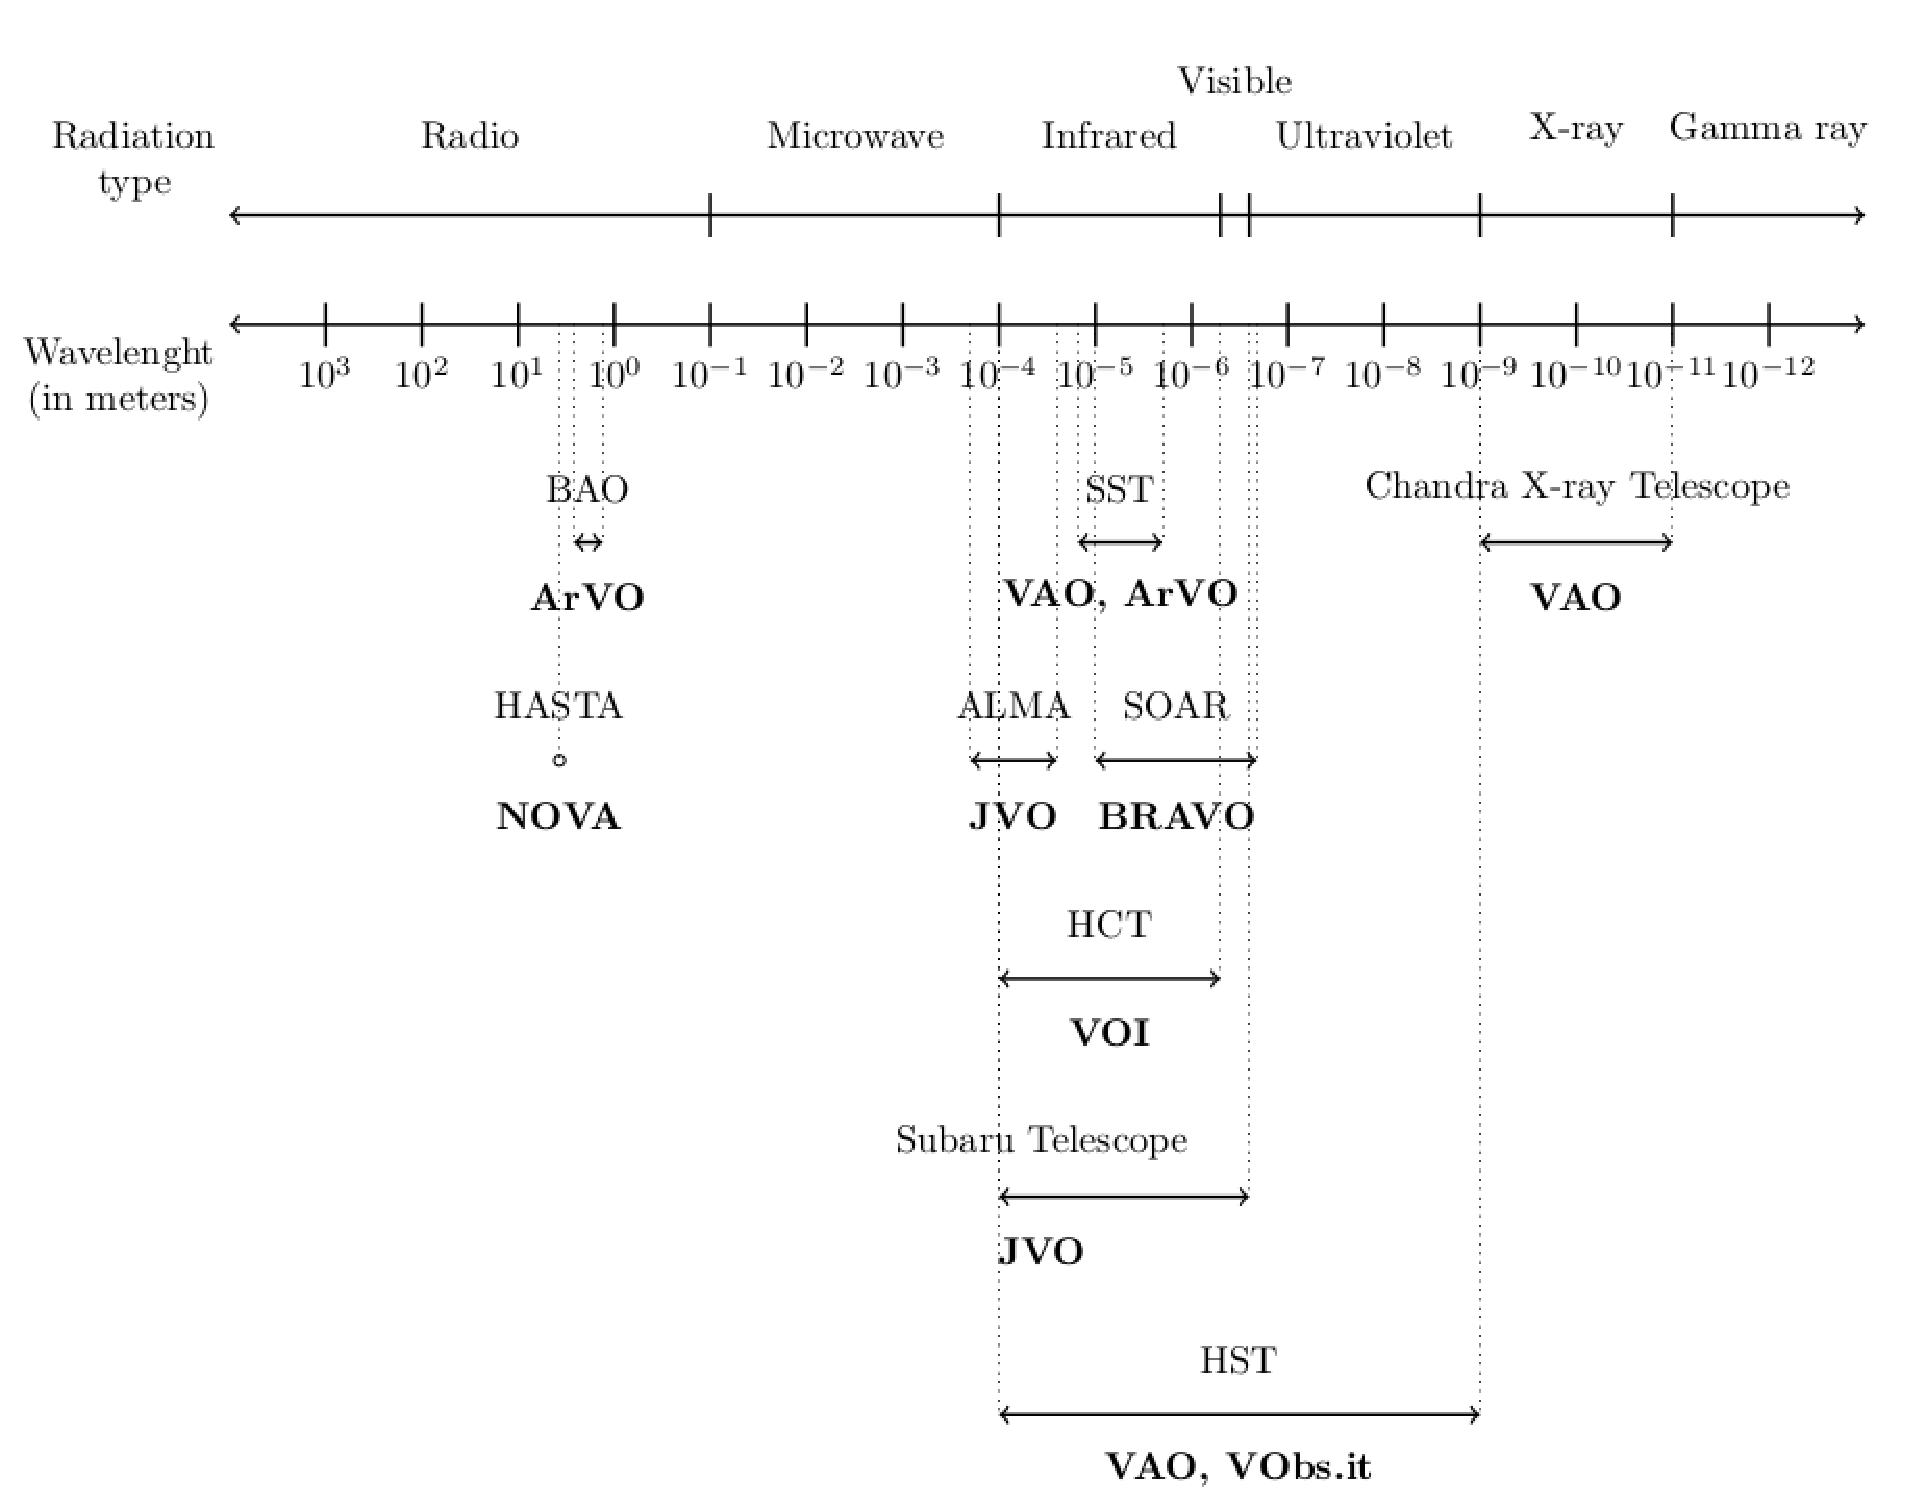
\includegraphics[width=0.85\textwidth]{img/wavebands}
                	\end{center}
	        \end{minipage}
      \end{kasten}

    \end{spalte}
     \hfill\mbox{}
}

\end{lrbox}
\hfill
\resizebox*{0.95\textwidth}{!}{
  \usebox{\spalten}}\hfill\mbox{}

\vspace{4.2cm}
\hspace{1cm}
\psshadowbox[cornersize=absolute,linearc=14pt]{\makebox[0.923\textwidth]{%
 \hfill
 \parbox[t]{0.9\linewidth}{
\begin{minipage}[t]{0.95\linewidth}
\section*{ {\normalsize \color{red} Conclusions}}
{%\footnotesize
			%\begin{minipage}[t]{0.90\linewidth}
This paper presents the IVOA architecture and the standards and protocols that
we use to the development of the Chilean Virtual Observatory. We presented the
state of the art of VOs and we summarized in a schematic diagram the frequency
range of the type of data that every VO publishes. In this diagram it is easy
to see that ALMA data will contribute and VO services will very helpfull to the
community. As a future work we are considering to have solid statistics to data
downloaded through ChiVO and access statistics of ChiVO services.%\vspace{1cm}
			%\end{minipage} \hspace{0.2cm}
}
\end{minipage}
}\hfill
}}\hfill\mbox{}\\
\vfill

\hfill
\psshadowbox{\makebox[0.95\linewidth]{
\hfill
\begin{minipage}[t]{0.30\linewidth}
	{\scriptsize
	{\small\bf Acknowledgements}
	
	\renewcommand{\baselinestretch}{0.4}
	This work is partially financed by the FONDEF D11I1060 project:
	``\emph{Development of an Astro-Informatic Platform for Management and Intelligent Analisys of Large-scale Data}''
	}
	
\end{minipage}\hfill

\begin{minipage}[t]{0.60\linewidth}
	{\scriptsize
	\renewcommand{\baselinestretch}{1.0}
	{\small\bf References}

        [1] Borne, K.D, ``Astroinformatics: a 21st century approach to astronomy'' (2009).
        \renewcommand{\baselinestretch}{0.5}

        [2] Tody, D. and Plante, R., ``Simple image access specification'' (2004). 
        \renewcommand{\baselinestretch}{0.5}

        [3] Williams, R., Hanisch, R., Szalay, A., and Plante, R., ``Simple cone search version 1.03'' (2008).
        \renewcommand{\baselinestretch}{0.5}

        [4] Tody, D., Dolensky, M., McDowell, J., Bonnarel, F., et al., ``Simple spectral access protocol'' (2008). 
        \renewcommand{\baselinestretch}{0.5}

        [5] Dowler, P., Rixon, G., Tody, D., Andrews, K., Good, J., J., Hanisch, R., Lemson, G., McGlynn, T., Noddle, et al ``Table access protocol version 1.0'' (2010).
        \renewcommand{\baselinestretch}{0.5}

        [6] Ochsenbein, F., Williams, R., Davenhall, C., DUrand, D., Fernique, P., Giaretta, et al, ``Votable format definition version 1.2'' (2011).
        \renewcommand{\baselinestretch}{0.5}
	}
\end{minipage}
}}\hfill\mbox{}

\hfill
\psshadowbox{\makebox[0.95\linewidth]{
\begin{minipage}[t]{0.15\linewidth}
	\begin{tabular}{cccc}
	\includegraphics[width=!,height=1.5cm]{logos/alma} &
	\includegraphics[width=!,height=1.5cm]{logos/fondef} &
	\includegraphics[width=!,height=1.5cm]{logos/utfsm} &
	\includegraphics[width=!,height=1.5cm]{logos/uchile} 
	\end{tabular}
\end{minipage} \hfill
\begin{minipage}[t]{0.50\linewidth}
	\begin{center}
	\Huge{Chilean Virtual Observatory}
	\end{center}
\end{minipage} \hfill
\begin{minipage}[t]{0.18\linewidth}
	\begin{tabular}{cccc}
	\includegraphics[width=!,height=1.5cm]{logos/puc}
	\includegraphics[width=!,height=1.5cm]{logos/reuna} &
	\includegraphics[width=!,height=1.5cm]{logos/udec} &
	\includegraphics[width=!,height=1.5cm]{logos/usach} &
	\end{tabular}
\end{minipage}
}}\hfill\mbox{}


\vfill
\hfill
{\scriptsize
Contact e-mail: {\color{blue}msolar@inf.utfsm.cl} / For more information about
Chilean Virtual Observatory, please visit our web site
{\color{blue}http://www.chivo.cl}
}
\hfill
\

\end{document}
